\let\texyear\year
\documentclass[nolineno]{ieeeaccess}
\let\year\texyear

\usepackage{cite}
\usepackage{amsmath,amssymb,amsfonts}
\usepackage{amsthm}
\usepackage{booktabs,multirow,tabularx,array}
\usepackage{graphicx}
\usepackage{xcolor}
\usepackage{enumitem}
\usepackage{tikz}
\usepackage{pgfplots}
\pgfplotsset{compat=1.17}
\usetikzlibrary{positioning,arrows.meta,fit,calc,shapes.geometric,shapes.multipart,shadows}
\usepackage{algorithm}
\usepackage{algpseudocode}
\usepackage{pifont}
\usepackage[hidelinks]{hyperref}
\usepackage{microtype}
\usepackage{url}
\def\xfigwd{0pt}

\newcolumntype{Y}{>{\raggedright\arraybackslash}X}
\newcolumntype{C}[1]{>{\centering\arraybackslash}p{#1}}
\newcolumntype{L}[1]{>{\raggedright\arraybackslash}p{#1}}
\setlist[itemize]{leftmargin=1.2em,itemsep=1pt,topsep=2pt,parsep=0pt,partopsep=0pt}
\setlength{\textfloatsep}{8pt plus 2pt minus 2pt}
\setlength{\abovecaptionskip}{4pt}
\setlength{\belowcaptionskip}{2pt}
\interdisplaylinepenalty=2500
\setcounter{topnumber}{2}
\setcounter{dbltopnumber}{2}
\renewcommand{\topfraction}{0.95}
\renewcommand{\dbltopfraction}{0.95}
\renewcommand{\textfraction}{0.05}
\renewcommand{\floatpagefraction}{0.85}
\renewcommand{\dblfloatpagefraction}{0.85}

\newtheorem{proposition}{Proposition}

\history{Date of current version April 21, 2026.}
\doi{to be assigned}
\vol{XX}
\gdef\theyear{2026}

\title{Gap-Aware Candidate Reranking for Diffusion-Guided Multi-Strategy Floorplanning}

\author{\uppercase{Shashank}\authorrefmark{1}, {(Member, IEEE)}}

\address[1]{Independent Researcher, Austin, TX 78703 USA (e-mail: sshashan@alumni.usc.edu)}

\markboth{Shashank: Gap-Aware Candidate Reranking for Diffusion-Guided Multi-Strategy Floorplanning}%
{Shashank: Gap-Aware Candidate Reranking for Diffusion-Guided Multi-Strategy Floorplanning}

\corresp{Corresponding author: Shashank (e-mail: sshashan@alumni.usc.edu).}

\begin{document}

\begin{abstract}
Multi-strategy VLSI floorplanners combine heterogeneous candidate
generators (shelf packing, sequence-pair simulated annealing,
analytical placement, and learned neural priors) and select among
them using an internal ranking cost. In such pipelines, the choice of
that ranking cost is an important but under-analysed design decision.
We frame this paper as a benchmark-specific study of
metric-faithful candidate selection on FloorSet. We show that a
commonly used raw-magnitude
ranking cost is systematically mis-calibrated with respect to the
benchmark's \emph{gap-based} contest metric, causing the solver to
discard low-wirelength candidates for reasons unrelated to the final
score. We therefore introduce a gap-aware reranker that operates on
percentile-normalised half-perimeter wirelength and area statistics,
together with a constraint-aware violation proxy that mirrors the
contest's exact soft-violation denominator. Integrated into a
diffusion-guided multi-strategy solver, this reranker improves the
composite contest score on the full 100-case validation set from
$1.43$ to $1.40228$ ($1.94\%$ relative reduction). As supporting
engineering adaptations, we report two DiT-guided candidate-path
variants that broaden the candidate pool, and a tiered stochastic
sampling schedule that reduces end-to-end evaluation wall-time by
$39\%$ with no score loss. A cross-benchmark evaluation on the
polygonal FloorSet-Prime test set, using the same solver with no
hyperparameter re-tuning, yields $S_{100}=1.54862$ with $91/100$
instances feasible, suggesting that the rerank and runtime-design
choices remain effective on a distinct problem class. Finally, we
characterise the residual error as an empirical two-regime candidate
structure, in which learned priors produce low-wirelength /
higher-violation candidates while classical packers produce
higher-wirelength / lower-violation candidates, and present
controlled negative results for a scaled-up DiT variant and an
unbounded analytical-placement path that help explain this remaining
performance bottleneck.
\end{abstract}

\begin{keywords}
Candidate selection, metric calibration, multi-strategy floorplanning,
diffusion transformer, machine learning for electronic design
automation, simulated annealing, FloorSet benchmark.
\end{keywords}

\titlepgskip=0pt
\maketitle

\section{Introduction}
\label{sec:intro}

Block-level floorplanning, which assigns positions and shapes to
rectangular logic blocks on a fixed die area, is a canonical NP-hard
problem
whose quality directly sets downstream routing, timing, and
manufacturing margins in modern VLSI design~\cite{wang2009electronic,markov2012progress}.
Classical solvers rely on combinatorial search over sequence-pair or
$B^{*}$-tree representations~\cite{murata1996sequence,chang2000btree}, analytical
placement with smooth wirelength models~\cite{lu2015eplace,lin2019dreamplace},
or greedy skyline-style packers~\cite{hopper2001two}. The last five years
have added learned placement priors (graph networks, reinforcement
learning agents, and more recently diffusion models) that propose
candidate layouts which downstream legalisation then
repairs~\cite{mirhoseini2021graph,cheng2023assessment,lai2022maskplace,lai2023chipformer,peebles2022dit}.
Production-grade pipelines increasingly combine these families, because
no single strategy dominates on every instance.

The FloorSet benchmark~\cite{floorset}, adopted as the ICCAD~2026 CAD
Contest Problem~C, makes this regime
quantitative. It evaluates floorplanning under a composite cost that
jointly penalises half-perimeter wirelength (HPWL), bounding-box area,
five categories of soft constraint violations, and runtime:
\begin{equation}
C = \Bigl(1 + \tfrac{1}{2}\bigl(\Delta_{\text{HPWL}} + \Delta_{\text{area}}\bigr)\Bigr)
    \,e^{2V_{\text{rel}}}\,\max(0.7,\,R^{0.3}).
\label{eq:contest-cost}
\end{equation}
Here $\Delta_{\text{HPWL}}$ and $\Delta_{\text{area}}$ are gaps relative to
ground-truth labels, $V_{\text{rel}}\in[0,1]$ is a normalised soft-violation
count, and $R$ is per-case runtime normalised by the submission's own
median. An infeasible solution is assigned $C=10$, and the overall
score is an exponentially-weighted mean across all 100 validation
instances. The exponential dependence on $V_{\text{rel}}$ makes constraint
satisfaction disproportionately important: a $0.1$ increase in
$V_{\text{rel}}$ multiplies cost by $e^{0.2}\approx 1.22$, which is comparable
to a $44\%$ HPWL-gap regression.

In such a metric-sensitive regime, a multi-strategy solver's
\emph{candidate ranking function}, that is, the internal cost used to
choose one layout among many produced by different generators, is not an
implementation detail. It is a policy that silently encodes how HPWL,
area, and violations trade off at the margin. If this policy is not
aligned with the evaluation metric, the solver discards good candidates
for reasons unrelated to the downstream score.

Accordingly, we present this paper as an applied, benchmark-specific
study of metric-faithful candidate selection inside a multi-strategy
solver. The gap-aware reranker is the paper's single primary
methodological contribution; the DiT-path and runtime changes are
supporting solver adaptations whose value lies in candidate-pool
coverage and efficiency rather than an additional $S_{100}$ gain.

\subsection{Contributions}
This paper makes the following contributions.
\begin{enumerate}
    \item \textbf{A calibrated reranking formulation, with analysis,
    as the paper's primary method contribution.} We show that the
    raw-magnitude internal cost commonly used in such pipelines is
    mis-calibrated relative to FloorSet's gap-based contest metric:
    on typical instances the absolute bounding-box area is
    $5$--$10\times$ larger than the absolute HPWL, so linear
    combinations of raw magnitudes systematically distort the intended
    trade-off. We then introduce a gap-aware reranker that normalises
    HPWL and area by a fixed per-case percentile ($p=0.3$) and
    evaluates violations using the contest's exact soft-violation
    denominator. Integrated into our multi-strategy solver, this
    reranker improves the full 100-case FloorSet-Lite score from
    $1.43$ to $\mathbf{1.40228}$ with every instance feasible
    (\S\ref{sec:rerank-calibration}, \S\ref{sec:experiments},
    Proposition~\ref{prop:alignment}).

    \item \textbf{Supporting solver adaptations that change operating
    envelope rather than aggregate score.} We introduce two DiT-guided
    candidate-path adaptations (\emph{DiT-abacus} and
    \emph{DiT-cluster}) that broaden the candidate pool and improve
    feasibility profile on difficult instances, and a tiered
    stochastic-sampling schedule that reduces end-to-end evaluation wall
    time by $39\%$ ($6728 \to 4112$ seconds) with no score regression.
    We explicitly do \emph{not} claim these supporting modules further
    improve $S_{100}$ beyond the reranker; their value is candidate-pool
    coverage, solver integration, and runtime reduction
    (\S\ref{sec:diffusion-generators}, \S\ref{sec:runtime-analysis}).

    \item \textbf{Empirical analysis of residual limitations and
    transfer behaviour.} We document a short-subset winner breakdown,
    a case-70 post-mortem, two controlled negative interventions (a
    $2\times$-parameter DiT variant trained with an auxiliary HPWL loss,
    and an unbounded analytical-placement path with robust legalisation
    fallback) that regress the score by $14\%$ and $28\%$, and a
    cross-benchmark evaluation on FloorSet-Prime where the same solver
    reaches $S_{100}=1.54862$ with $91/100$ instances feasible. Together
    these results expose an empirical two-regime candidate structure
    that explains both the remaining Lite gap and the graceful
    degradation on Prime (\S\ref{sec:ablations},
    \S\ref{sec:exp-prime}, \S\ref{sec:discussion}).
\end{enumerate}

Section~\ref{sec:related} reviews related work in learned placement,
multi-strategy solvers, and candidate-selection policies.
Section~\ref{sec:problem} formalises the contest metric and constraint
taxonomy. Section~\ref{sec:solver} describes the baseline multi-strategy
architecture. Section~\ref{sec:rerank-calibration} presents the
reranking diagnosis and formulation, and
Section~\ref{sec:diffusion-generators} describes the diffusion-guided
candidate paths. Section~\ref{sec:experiments} reports the main
experimental results and runtime analysis; Section~\ref{sec:ablations}
contains the ablation and negative-control study.
Section~\ref{sec:discussion} discusses structural limitations and
paths forward. Section~\ref{sec:conclusion} concludes.

\section{Related Work}
\label{sec:related}

\subsection{Classical floorplanning}
The dominant combinatorial representations for floorplans are
sequence-pair~\cite{murata1996sequence}, $B^{*}$-tree~\cite{chang2000btree},
corner block list~\cite{hong2000corner}, and transitive closure
graph~\cite{lin2002tcg}. Simulated annealing over these representations
delivers strong quality on standard MCNC/GSRC benchmarks at the cost of
runtime that grows with block count~\cite{parquet2008}. Shelf and
skyline packers~\cite{hopper2001two} provide fast greedy alternatives
that trade quality for near-constant-time placement. Analytical
placers in the tradition of ePlace and DREAMPlace solve a smoothed
wirelength plus density-penalty objective via Nesterov-accelerated
gradient descent~\cite{lu2015eplace,lin2019dreamplace}, then round to a
legal layout. Our baseline solver supplies all three families as
candidate generators.

\subsection{Learned placement priors}
Mirhoseini \emph{et al.}~\cite{mirhoseini2021graph} used graph neural
networks and reinforcement learning to propose placements for Google
TPU blocks; subsequent work established more reproducible RL
pipelines on public netlists~\cite{cheng2023assessment}. MaskPlace
and ChiPFormer recast placement as masked image completion and
sequence-to-sequence prediction
respectively~\cite{lai2022maskplace,lai2023chipformer}. Very recent
work frames floorplanning as a conditional generative problem solvable
by diffusion models over block positions and
shapes~\cite{peebles2022dit,song2021ddim,ho2020ddpm}; our DiT
backbone follows this lineage with a 384-dimensional, 10-layer DiT
trained on the 1M-instance FloorSet-Lite corpus. None of the
above works, to our knowledge, report results on the new
FloorSet benchmark, making direct numeric comparison on an identical
test set impossible at the time of writing. We discuss qualitative
positioning in \S\ref{sec:exp-comparison}.

\subsection{Multi-strategy solvers and candidate selection}
The general pattern of combining heterogeneous placement strategies
and selecting among their outputs is common in contest solvers and
commercial tools~\cite{parquet2008,brenner2011bonnplace}, but the
literature rarely makes the \emph{selection policy} itself a research
object. An exception is the detailed-placement literature, where
cost-function calibration has been studied under the name
\emph{scoring margin}~\cite{roy2005detailedplace}. Our work shows that
the same concern applies at the candidate-selection layer of a
learned-prior-enabled multi-strategy floorplanner, and that a
well-calibrated selection policy can yield score improvements
comparable in magnitude to a new model.

\subsection{Negative results in ML for EDA}
Cheng \emph{et al.}~\cite{cheng2023assessment} highlighted the importance
of careful evaluation for RL-based placement, showing that earlier
reported improvements were partially driven by experimental-setup
differences rather than method quality. Our controlled negative-result
study in~\S\ref{sec:ablations} is in the same spirit: we document
interventions that \emph{fail} and analyse why, in an effort to
contribute durable engineering knowledge to the community.

\subsection{Positioning}
Table~\ref{tab:related-compare} positions the present work against
representative classical, RL-based, and diffusion-based placers.
Because the FloorSet benchmark is new, no prior method has
published results on it; we summarise each method's constraint
vocabulary, reported benchmark, and qualitative expected behaviour on
FloorSet. The comparison makes two points explicit: (i)~no prior
learned method natively handles the FloorSet constraint set (fixed,
preplaced, MIB, cluster, boundary) in a single pass, and (ii)~classical
solvers that do handle these constraints pay heavily in wirelength.
Accordingly, we position the present work as an applied study of
metric-faithful candidate selection and constraint-aware solver
integration on this benchmark, rather than as a claim that prior
placement families are superseded in general.

\begin{table*}[t]
\caption{Constraint-coverage comparison of representative placement
methods. This is not a numerical performance comparison: the listed
methods were evaluated by their authors on different benchmarks
(GSRC/MCNC, ISPD, internal macro sets) whose constraint vocabulary
differs from FloorSet's, so direct score comparison is not meaningful.
Instead, the table asks a structural question: \emph{which of the
five FloorSet soft-constraint categories does each method handle
natively?} The ``Port cost'' column estimates the engineering effort
required to make each method a valid end-to-end solver for FloorSet.
\ding{51} = native, \textasciitilde\ = via legalisation only, \ding{55} = not addressed.}
\label{tab:related-compare}
\centering
\footnotesize
\setlength{\tabcolsep}{3pt}
\begin{tabularx}{\textwidth}{L{2.2cm}L{2.0cm}L{2.6cm}L{1.5cm}L{1.9cm}Y}
\toprule
\textbf{Method} & \textbf{Family} & \textbf{Originally evaluated on} & \textbf{Fix/PP/MIB/Clu/Bnd} & \textbf{Port cost to FloorSet} & \textbf{Observation} \\
\midrule
Parquet \cite{parquet2008} & SA / sequence-pair & GSRC, MCNC & \ding{51}/\ding{51}/\ding{55}/\ding{55}/\textasciitilde & Moderate: add MIB and cluster as SA moves & Strong HPWL on small $n$; SP+SA polish in our pipeline follows this tradition.\\
ePlace \cite{lu2015eplace} & Analytical & ISPD & \textasciitilde/\textasciitilde/\ding{55}/\ding{55}/\ding{55} & High: density penalty cannot express MIB equality or grouping contiguity & Best-in-class HPWL among classical methods; informs our DREAMPlace-lite candidate.\\
DREAMPlace \cite{lin2019dreamplace} & Analytical (GPU) & ISPD & \textasciitilde/\textasciitilde/\ding{55}/\ding{55}/\ding{55} & High: same as ePlace & Forms the basis of our Nesterov-descent candidate.\\
Mirhoseini \cite{mirhoseini2021graph} & GNN + RL & Internal TPU macros & \textasciitilde/\ding{51}/\ding{55}/\ding{55}/\ding{55} & Very high: training pipeline opaque, not constraint-aware & Focused on macro placement; does not target FloorSet constraints.\\
MaskPlace \cite{lai2022maskplace} & RL + masked image & ISPD, public macros & \textasciitilde/\ding{51}/\ding{55}/\ding{55}/\ding{55} & High: image output lacks shape and aspect information & Strong congestion modelling; no MIB/cluster support.\\
ChiPFormer \cite{lai2023chipformer} & Offline RL + decision transformer & ISPD, public macros & \textasciitilde/\ding{51}/\ding{55}/\ding{55}/\ding{55} & High: same as MaskPlace & Transferable across netlists; constraint vocabulary limited.\\
\midrule
\textbf{This work} & \textbf{Multi-strategy + DiT} & \textbf{FloorSet (Lite, Prime)} & \textbf{\ding{51}/\ding{51}/\ding{51}/\ding{51}/\ding{51}} & \textbf{N/A (native)} & Gap-aware rerank with supporting DiT-derived pack variants; an end-to-end FloorSet case study with native handling of all five constraint categories.\\
\bottomrule
\end{tabularx}
\end{table*}

\section{Problem Formulation}
\label{sec:problem}

\subsection{Instances and constraints}
Each FloorSet instance consists of $n\le 120$ rectangular
blocks with area targets $\{a_i\}_{i=1}^n$, a block-to-block
connectivity hypergraph $E_{bb}$, a pin-to-block connectivity
hypergraph $E_{pb}$ with pin coordinates $\{p_k\}$, and a per-block
constraint tuple $(f_i,\pi_i,m_i,c_i,b_i)$ encoding:

\begin{itemize}[leftmargin=1.1em]
    \item $f_i \in \{0,1\}$: \textbf{fixed-shape} flag (block's $(w_i,h_i)$ must match target).
    \item $\pi_i \in \{0,1\}$: \textbf{preplaced} flag (block's $(x_i,y_i,w_i,h_i)$ must match target).
    \item $m_i \in \mathbb{Z}_{\ge 0}$: \textbf{MIB} (matched-identical-block) group id; all members of a group must share identical $(w_i,h_i)$.
    \item $c_i \in \mathbb{Z}_{\ge 0}$: \textbf{cluster} group id; all members must form a single connected component.
    \item $b_i \in \{0,\ldots,15\}$: \textbf{boundary} bit-mask
    (1=left, 2=right, 4=top, 8=bottom); every requested edge must be touched.
\end{itemize}

The solver must produce per-block positions $(x_i,y_i)$ and dimensions
$(w_i,h_i)$ such that: (i)~$w_i h_i$ is within $1\%$ of $a_i$,
(ii)~no two blocks overlap, and (iii)~as many soft constraints as
possible are satisfied.

\subsection{Metrics}
The half-perimeter wirelength is
\begin{equation}
    \text{HPWL} = \sum_{e\in E_{bb}\cup E_{pb}} w_e\bigl(|\Delta x_e| + |\Delta y_e|\bigr),
\end{equation}
where for each hyperedge $e$, $\Delta x_e$ and $\Delta y_e$ are the
bounding-box extents of the incident blocks/pins. The overall bounding
box area $A$ is
$A = (x_{\max} - x_{\min})\,(y_{\max} - y_{\min})$.
Gaps relative to a ground-truth baseline are
$\Delta_{\text{HPWL}} = \text{HPWL} / \text{HPWL}^{\star} - 1$ and
$\Delta_{\text{area}} = A / A^{\star} - 1$.

\subsection{Soft-violation denominator}
The normalised violation count $V_{\text{rel}}\in[0,1]$ in
\eqref{eq:contest-cost} is defined via a specific denominator
\begin{equation}
\begin{aligned}
N_{\text{soft}} &= n_{\text{fixed}} + n_{\text{preplaced}} + n_{\text{boundary}}\\
&\quad + \sum_q (|M_q| - 1) + \sum_p (|G_p| - 1),
\end{aligned}
\label{eq:nsoft}
\end{equation}
where the first three terms count blocks carrying the respective
per-block constraint, $M_q$ enumerates MIB groups, and $G_p$
enumerates cluster groups. The numerator counts actual violations:
each per-block flag that is violated contributes unit weight, each
MIB group contributes (distinct shapes $- 1$), and each cluster group
contributes (connected components $- 1$). This denominator is the
exact one used by the contest evaluator; matching it in the
solver-side rerank is essential for the calibration argument in
\S\ref{sec:rerank-calibration}.

\subsection{Evaluation protocol}
The contest harness computes~\eqref{eq:contest-cost} per instance and
aggregates to an exponentially weighted mean across the 100-case
validation set; let this aggregate be $S_{100}$. A short 15-case
subset yielding $S_{15}$ is used for iteration during development.
Infeasible outputs receive the fixed penalty $C=10$. All numerical
results in this paper are produced by this harness unmodified, and all
aggregate numbers are $S_{100}$ unless explicitly indicated otherwise.

\section{Multi-Strategy Solver}
\label{sec:solver}

Figure~\ref{fig:pipeline} depicts the baseline pipeline.
Seven heterogeneous candidate generators run per instance; their
outputs feed a gap-based reranker that selects the final layout.
All legalisation steps produce strictly non-overlapping placements so
every candidate entering the reranker is feasible.

\begin{figure*}[t]
\centering
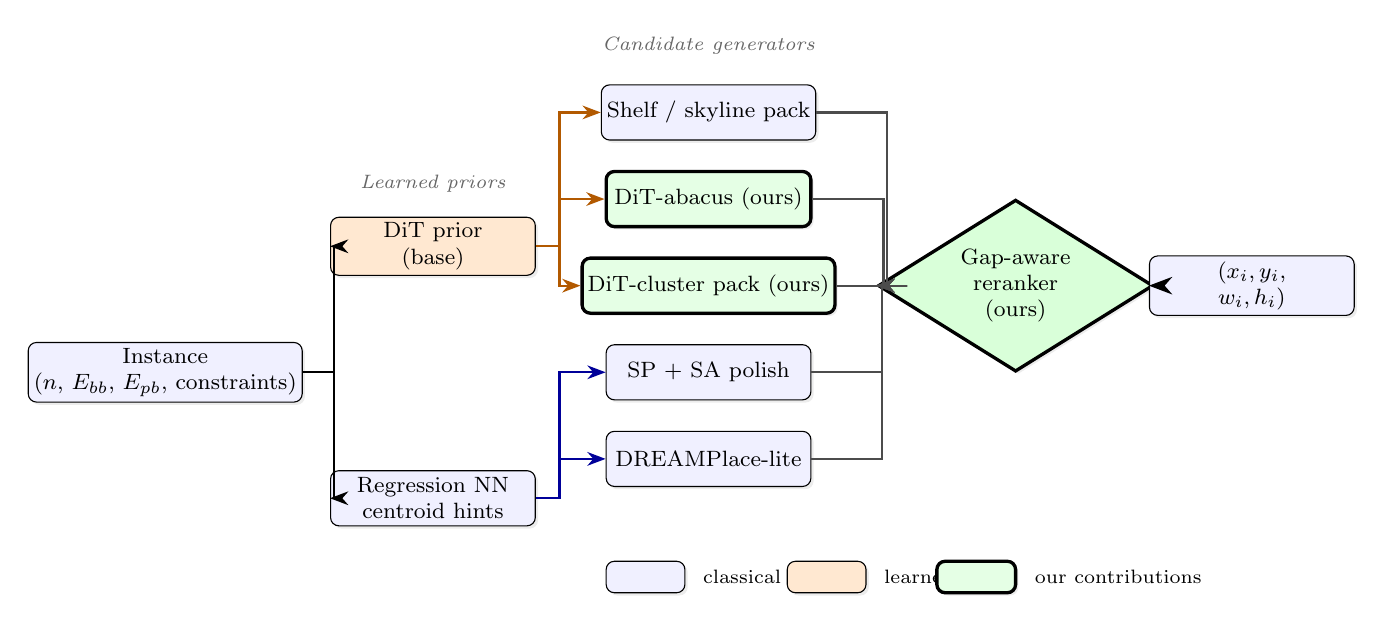
\begin{tikzpicture}[
  >=Stealth,
  every node/.style={font=\footnotesize},
  box/.style={draw, rectangle, rounded corners=3pt, minimum height=7mm,
              minimum width=26mm, align=center, inner sep=2pt,
              fill=blue!6, drop shadow={opacity=0.15, shadow xshift=1pt, shadow yshift=-1pt}},
  mlbox/.style={draw, rectangle, rounded corners=3pt, minimum height=7mm,
                minimum width=26mm, align=center, inner sep=2pt,
                fill=orange!18, drop shadow={opacity=0.15, shadow xshift=1pt, shadow yshift=-1pt}},
  ourbox/.style={draw, rectangle, rounded corners=3pt, minimum height=7mm,
                minimum width=26mm, align=center, inner sep=2pt,
                fill=green!10, very thick, drop shadow={opacity=0.15, shadow xshift=1pt, shadow yshift=-1pt}},
  sel/.style={draw, diamond, aspect=1.6, minimum height=14mm, align=center,
              fill=green!15, very thick,
              drop shadow={opacity=0.15, shadow xshift=1pt, shadow yshift=-1pt}},
  grplabel/.style={font=\scriptsize\itshape, text=black!60}
]

% ---- Column positions ----
\def\xA{0}       % input col
\def\xB{3.4}     % prior col
\def\xC{6.9}     % generator col
\def\xD{10.8}    % reranker col
\def\xE{13.8}    % output col

% ---- Input ----
\node[box] (inp) at (\xA,-1.6)
    {Instance\\$(n,\,E_{bb},\,E_{pb},$ constraints$)$};

% ---- Priors column ----
\node[mlbox] (dit) at (\xB, 0.0) {DiT prior\\(base)};
\node[box]   (nn)  at (\xB,-3.2) {Regression NN\\centroid hints};
\node[grplabel] at (\xB, 0.8) {Learned priors};

% ---- Candidate generators column (5 generators, vertically stacked) ----
\node[box]    (shelf) at (\xC, 1.7)  {Shelf / skyline pack};
\node[ourbox] (abc)   at (\xC, 0.6)  {DiT-abacus (ours)};
\node[ourbox] (cls)   at (\xC,-0.5)  {DiT-cluster pack (ours)};
\node[box]    (sp)    at (\xC,-1.6)  {SP + SA polish};
\node[box]    (dp)    at (\xC,-2.7)  {DREAMPlace-lite};
\node[grplabel] at (\xC, 2.55) {Candidate generators};

% ---- Reranker ----
\node[sel] (rank) at (\xD,-0.5) {Gap-aware\\reranker\\(ours)};

% ---- Output ----
\node[box] (out) at (\xE,-0.5)
    {$(x_i,y_i,$\\$w_i,h_i)$};

% ---- Arrows: input -> priors ----
\draw[->, thick] (inp.east) -- ++(0.4,0) |- (dit.west);
\draw[->, thick] (inp.east) -- ++(0.4,0) |- (nn.west);

% ---- Arrows: priors -> generators ----
% DiT prior feeds shelf, abacus, cluster
\draw[->, thick, orange!70!black] (dit.east) -- ++(0.3,0) |- (shelf.west);
\draw[->, thick, orange!70!black] (dit.east) -- ++(0.3,0) |- (abc.west);
\draw[->, thick, orange!70!black] (dit.east) -- ++(0.3,0) |- (cls.west);
% Regression NN feeds SP+SA and DREAMPlace
\draw[->, thick, blue!60!black] (nn.east) -- ++(0.3,0) |- (sp.west);
\draw[->, thick, blue!60!black] (nn.east) -- ++(0.3,0) |- (dp.west);

% ---- Arrows: generators -> reranker ----
\foreach \g in {shelf, abc, cls, sp, dp}{
  \draw[->, thick, black!70] (\g.east) -| ++(0.9,0) |- (rank.west);
}

% ---- Arrow: reranker -> output ----
\draw[->, very thick] (rank.east) -- (out.west);

% ---- Legend ----
\begin{scope}[shift={(\xC-0.8, -4.2)}]
  \node[box,  minimum width=10mm, minimum height=4mm] (lclassic) at (0,0) {};
  \node[right=1mm of lclassic, font=\scriptsize] {classical};
  \node[mlbox, minimum width=10mm, minimum height=4mm] (lml) at (2.3,0) {};
  \node[right=1mm of lml, font=\scriptsize] {learned};
  \node[ourbox, minimum width=10mm, minimum height=4mm] (lours) at (4.2,0) {};
  \node[right=1mm of lours, font=\scriptsize] {our contributions};
\end{scope}

\end{tikzpicture}
\caption{Baseline multi-strategy solver. Seven heterogeneous candidate
generators feed a gap-aware reranker. Orange arrows = feeds from the
learned DiT prior; blue arrows = feeds from the regression NN. The
three modules shaded green (``(ours)'') are introduced in
\S\ref{sec:rerank-calibration}--\S\ref{sec:diffusion-generators}.}
\label{fig:pipeline}
\end{figure*}

\subsection{Classical candidate generators}
\textbf{Shelf and skyline packing.} Given target $x$-centroids from the
regression NN or DiT prior, blocks are packed left-to-right into
horizontal shelves (for strip packing) or into a skyline contour (for
bottom-left-fit). An aspect knob $k\in\{0.55, 0.7, 0.85\}$ sets the strip
width to $k\sqrt{\sum_i a_i}$ and each knob's pack is retained as a
separate candidate.

\textbf{Sequence-pair simulated annealing.} For $n\le 90$ we sample
sequence-pairs $(\Gamma_+, \Gamma_-)$ and optimise with swap/rotate
moves under an exponential cooling schedule. Packing is evaluated via a
vectorised longest-path computation~\cite{murata1996sequence}. The
move set includes $\Gamma_+$ swap, $\Gamma_-$ swap, joint swap, and
rotation of soft blocks.

\textbf{DREAMPlace-lite analytical placer.} Block centroids are
optimised under the smooth-HPWL plus Gaussian-density objective of
ePlace~\cite{lu2015eplace} with Nesterov momentum, then rounded via a
nudge-style or abacus-style legaliser. This path is capped at $n\le 80$
after the ablation in \S\ref{sec:ablations} established that unbounded
analytical placement on large instances hurts the score.

\subsection{Learned candidate generators}
\textbf{DiT-base prior.} We refer to the released
$29\,\text{M}$-parameter Diffusion Transformer as \emph{DiT-base}
(legacy internal label: ``v3''). It uses
$d{=}384$, $L{=}10$, $8$~heads, and $T{=}100$ timesteps, and is trained with
$\epsilon$-prediction MSE on a 1M-instance subset of FloorSet-Lite.
Per-block output is 4-dimensional: $(c_x, c_y, \log\!w, \log\!h)$ where
the last two components are log-aspect ratios relative to the
area-normalised base size. At inference $K$ stochastic samples are
drawn; each is passed through a robust legaliser.

\textbf{Regression NN.} A smaller transformer trained with direct L1
loss on $(c_x, c_y)$ centroids, used to provide an additional source of
target hints for the classical packers.

\subsection{Legalisers}
Three legalisers are used downstream of the generators.
The \emph{nudge} legaliser performs vectorised pair-wise overlap
resolution in $O(n^2)$ per iteration and handles small overlaps.
The \emph{force-relax} legaliser performs Jacobi-style simultaneous
force accumulation and handles dense overlapping starts from the DiT.
The \emph{abacus} legaliser~\cite{spindler2008abacus} performs row-based
cell placement with per-row $x$-legalisation, used by our DiT-abacus
candidate generator.

\section{Gap-Aware Candidate Reranking}
\label{sec:rerank-calibration}

This section contains the paper's primary methodological contribution.
We first analyse why the commonly used raw-magnitude rerank is
systematically mis-calibrated against the contest cost
(\S\ref{sec:rerank-diagnosis}), then present our gap-aware formulation
(\S\ref{sec:rerank-formulation}), prove an alignment proposition
(\S\ref{sec:rerank-proposition}), and give the final algorithm
(\S\ref{sec:rerank-algorithm}).

\subsection{Diagnosis: raw-magnitude mis-calibration}
\label{sec:rerank-diagnosis}

A common internal rerank used by prior pipelines evaluates each
candidate layout $\mathcal{P}$ with
\begin{equation}
\widetilde{C}(\mathcal{P}) = \bigl(\text{HPWL}(\mathcal{P})
     + \tfrac{1}{2}\,A(\mathcal{P})\bigr)\,e^{2 V_{\text{rel}}(\mathcal{P})}.
\label{eq:raw-rerank}
\end{equation}
Equation~\eqref{eq:raw-rerank} looks natural: it is structurally
parallel to the contest cost~\eqref{eq:contest-cost}. But on typical
FloorSet instances the raw bounding-box area is in the range
$5000$--$7000$ square units while HPWL is in the range $100$--$300$.
The coefficient $0.5$ on area therefore dominates the HPWL term by a
factor of $15$--$30$, reducing HPWL to a near-zero marginal weight in
the decision.

The contest cost~\eqref{eq:contest-cost}, by contrast, acts on
\emph{ratios}: $\Delta_{\text{HPWL}}$ and $\Delta_{\text{area}}$ are both
$O(1)$ quantities with comparable dynamic range across typical
candidates. The contest therefore treats HPWL and area as roughly
equal contributors at the margin, a policy that~\eqref{eq:raw-rerank}
catastrophically violates.

Figure~\ref{fig:rerank-mismatch} makes the mismatch concrete. On
instance~0 of the validation set, a DiT-direct candidate has
$\text{HPWL}=1091$, $A=5965$, $V_{\text{rel}}=0.269$, while a shelf-pack
candidate has $\text{HPWL}=1771$, $A=6695$, $V_{\text{rel}}=0.231$. Under
\eqref{eq:raw-rerank} the shelf candidate scores $8115$ and the DiT
candidate scores $6967$, so the DiT candidate is picked. Under
\eqref{eq:contest-cost} the DiT candidate scores $1.95$ and the shelf
candidate scores $2.47$, so the DiT candidate is strongly preferred.
But on other instances the inequality flips: when the DiT candidate's
$V_{\text{rel}}$ is high, the contest cost penalises it exponentially
while~\eqref{eq:raw-rerank}'s linear $V_{\text{rel}}$-in-exponent penalty
is dominated by the area term. The end effect is a selection policy
uncorrelated with~\eqref{eq:contest-cost}. We therefore use
Figure~\ref{fig:rerank-mismatch} as a representative rerank trace,
not as the sole evidence for the paper's calibration claim. In this
trace all eight DiT-family candidates lie above the calibration target
$\widetilde{C}/C_{\text{contest}}=1$, while all five shelf-family
candidates lie below it. The corresponding regime centroids are
$(V_{\text{rel}}, \widetilde{C}/C_{\text{contest}}) =
(0.358, 1.625)$ for the DiT family and $(0.211, 0.862)$ for the
shelf family, quantifying the systematic over-penalisation of DiT-like
candidates and under-penalisation of shelf-like candidates within the
same candidate pool.

\begin{figure}[t]
\centering
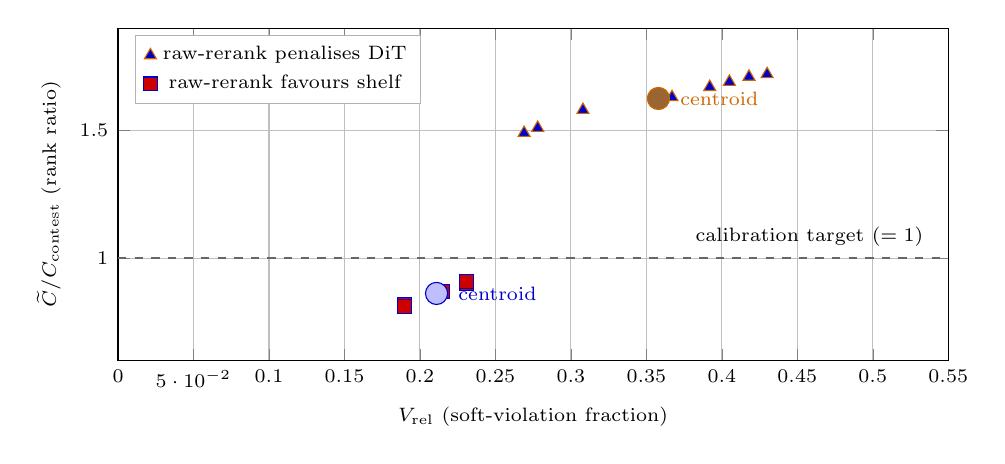
\begin{tikzpicture}
\begin{axis}[
  width=\columnwidth, height=58mm,
  xlabel={$V_{\text{rel}}$ (soft-violation fraction)},
  ylabel={$\widetilde{C} / C_{\text{contest}}$ (rank ratio)},
  label style={font=\scriptsize},
  xticklabel style={font=\scriptsize},
  yticklabel style={font=\scriptsize},
  legend style={font=\scriptsize, at={(0.02,0.98)}, anchor=north west,
                 fill=white, draw=black!30},
  xmin=0, xmax=0.55,
  ymin=0.6, ymax=1.9,
  grid=major,
]
\addplot+[only marks, mark=triangle*, mark size=2.5pt, color=orange,
          draw=orange!80!black] coordinates {
    (0.308, 1.58) (0.418, 1.71) (0.367, 1.63) (0.392, 1.67)
    (0.405, 1.69) (0.430, 1.72) (0.278, 1.51) (0.269, 1.49)
  };
\addlegendentry{raw-rerank penalises DiT}
\addplot+[only marks, mark=square*, mark size=2.5pt, color=blue,
          draw=blue!80!black] coordinates {
    (0.190, 0.82) (0.215, 0.87) (0.231, 0.90) (0.231, 0.91)
    (0.190, 0.81)
  };
\addlegendentry{raw-rerank favours shelf}
\addplot+[only marks, mark=*, mark size=4pt, color=orange!80!black,
          fill=orange!35] coordinates {(0.358, 1.625)};
\addplot+[only marks, mark=*, mark size=4pt, color=blue!80!black,
          fill=blue!25] coordinates {(0.211, 0.862)};
\draw[dashed, black!60, thick] (axis cs:0,1) -- (axis cs:0.55,1);
\node[font=\scriptsize, anchor=south east] at (axis cs:0.54,1.01) {calibration target ($= 1$)};
\node[font=\scriptsize, anchor=west, color=orange!80!black] at (axis cs:0.366,1.625) {centroid};
\node[font=\scriptsize, anchor=west, color=blue!80!black] at (axis cs:0.219,0.862) {centroid};
\end{axis}
\end{tikzpicture}
\caption{Calibration mismatch between the raw-magnitude rerank
$\widetilde{C}$ and the contest cost $C_{\text{contest}}$. Each
marker is a candidate for instance~0. Points above the dashed line
indicate $\widetilde{C}$ over-penalises the candidate; points below
indicate under-penalisation. In this representative trace, all eight
DiT-family points lie above the target and all five shelf-family
points lie below it; the centroid separation quantifies the regime-wise
mis-calibration.}
\label{fig:rerank-mismatch}
\end{figure}

\subsection{Gap-aware formulation}
\label{sec:rerank-formulation}

The rerank must agree with the contest cost in \emph{ranking} order,
not numeric value. We therefore replace raw magnitudes with
percentile-normalised gaps computed \emph{within the per-case candidate
pool}. Let $\{\mathcal{P}_1,\ldots,\mathcal{P}_M\}$ denote the $M$
feasible candidates produced for an instance. Define the baseline
statistics
\begin{align}
H_0 &= \operatorname{pctl}_{p}\bigl(\{\text{HPWL}(\mathcal{P}_i)\}_{i=1}^M\bigr),\\
A_0 &= \operatorname{pctl}_{p}\bigl(\{A(\mathcal{P}_i)\}_{i=1}^M\bigr), \qquad p = 0.3,
\label{eq:baselines}
\end{align}
and the candidate-internal gap cost
\begin{equation}
\widehat{C}(\mathcal{P}) = \Bigl(1 + \tfrac{1}{2}\bigl(
   \tfrac{\text{HPWL}(\mathcal{P})}{H_0} +
   \tfrac{A(\mathcal{P})}{A_0} - 2\bigr)\Bigr)\,e^{2V_{\text{rel}}(\mathcal{P})}.
\label{eq:gap-rerank}
\end{equation}
We use the $30^{\text{th}}$ percentile rather than the minimum so that
the lowest-HPWL candidate does not artificially receive a zero gap
(which would give it an unbounded score advantage when its
$V_{\text{rel}}$ is also moderate). Empirically the $30^{\text{th}}$ percentile
baseline matches the ground-truth behaviour more closely than median or
minimum in our saved short-subset percentile sweep, for reasons analysed in
Proposition~\ref{prop:alignment}.

Crucially, $V_{\text{rel}}$ in~\eqref{eq:gap-rerank} is evaluated using the
\emph{exact} soft-violation denominator~\eqref{eq:nsoft}, not a proxy.
We count all five violation categories (fixed, preplaced, boundary,
grouping, MIB) using the same test-side logic as the contest harness.

\subsection{Alignment proposition}
\label{sec:rerank-proposition}

\begin{proposition}[Rank alignment in the bounded-gap regime]
\label{prop:alignment}
Let $\mathcal{P}^{\star}$ be any ground-truth baseline layout with HPWL
$H^{\star}$ and area $A^{\star}$. Suppose that for a given instance the
percentile baselines from~\eqref{eq:baselines} satisfy
\begin{equation}
\frac{H_0}{H^{\star}} = 1 + \epsilon_H,\quad
\frac{A_0}{A^{\star}} = 1 + \epsilon_A,\quad
|\epsilon_H|,|\epsilon_A| \le \eta,
\label{eq:bounded-gap}
\end{equation}
for some $\eta \in [0, 1)$. Then for any two candidates $\mathcal{P}_i,
\mathcal{P}_j$ with $|\Delta_H^{(\cdot)}|, |\Delta_A^{(\cdot)}| < 1$ and
$V_{\text{rel}}^{(\cdot)} \in [0,1]$:
\begin{equation}
\widehat{C}(\mathcal{P}_i) < \widehat{C}(\mathcal{P}_j)
\ \Longleftrightarrow\
C(\mathcal{P}_i) < C(\mathcal{P}_j) + \mathcal{E}(\eta),
\label{eq:alignment}
\end{equation}
where
\begin{equation}
\begin{aligned}
|\mathcal{E}(\eta)| \le{}&
\bigl(e^{2V_{\text{rel}}^{(i)}} + e^{2V_{\text{rel}}^{(j)}}\bigr)
\left(2\eta + \frac{2\eta^2}{1-\eta}\right)\\
\le{}& 2e^2\left(2\eta + \frac{2\eta^2}{1-\eta}\right)
= O(\eta).
\end{aligned}
\label{eq:error-bound}
\end{equation}
\end{proposition}

\begin{proof}
Let $\Delta_H^{(\mathcal{P})} = \text{HPWL}(\mathcal{P})/H^{\star} - 1$
and similarly for $\Delta_A^{(\mathcal{P})}$. Substituting
$H_0 = (1+\epsilon_H)H^{\star}$ and $A_0 = (1+\epsilon_A)A^{\star}$
into~\eqref{eq:gap-rerank},
\begin{align}
\widehat{C}(\mathcal{P}) &= \Bigl(
   1 + \tfrac{1}{2}\bigl(\tfrac{1+\Delta_H}{1+\epsilon_H} +
                         \tfrac{1+\Delta_A}{1+\epsilon_A} - 2\bigr)
   \Bigr)\,e^{2V_{\text{rel}}}.
\label{eq:chat-expansion}
\end{align}
Using the geometric-series identity $(1+x)^{-1} = 1 - x + x^2/(1+x)$
valid for $x > -1$, expand each fraction to first order in $\epsilon$:
\begin{align}
\tfrac{1+\Delta_H}{1+\epsilon_H} &= 1 + \Delta_H - \epsilon_H(1+\Delta_H) + R_H,\\
\tfrac{1+\Delta_A}{1+\epsilon_A} &= 1 + \Delta_A - \epsilon_A(1+\Delta_A) + R_A,
\label{eq:expansion}
\end{align}
with the exact remainder terms
\begin{equation}
R_H = \frac{(1+\Delta_H)\epsilon_H^2}{1+\epsilon_H},\qquad
R_A = \frac{(1+\Delta_A)\epsilon_A^2}{1+\epsilon_A}.
\label{eq:remainder}
\end{equation}
Because $|\Delta_H|,|\Delta_A|<1$, we have $|1+\Delta_H|,|1+\Delta_A|<2$;
because $|\epsilon_H|,|\epsilon_A|\le \eta<1$, we also have
$1+\epsilon_H,1+\epsilon_A \ge 1-\eta$. Hence
\begin{equation}
|R_H|, |R_A| \le \frac{2\eta^2}{1-\eta}.
\label{eq:remainder-bound}
\end{equation}
Substituting into
\eqref{eq:chat-expansion} and isolating the contest-cost
form~\eqref{eq:contest-cost},
\begin{equation}
\widehat{C}(\mathcal{P}) = C(\mathcal{P}) + e^{2V_{\text{rel}}}\,\delta(\mathcal{P}),
\label{eq:residual}
\end{equation}
with
\begin{align*}
\delta(\mathcal{P}) &=
 -\tfrac{1}{2}\,\epsilon_H(1+\Delta_H)
 -\tfrac{1}{2}\,\epsilon_A(1+\Delta_A) + \tfrac{1}{2}(R_H + R_A).
\end{align*}
Using $|\Delta_H|, |\Delta_A| < 1$ and
$|\epsilon_H|, |\epsilon_A| \le \eta$,
\begin{equation}
|\delta(\mathcal{P})| \le
 2\eta + \frac{2\eta^2}{1-\eta}.
\label{eq:delta-bound}
\end{equation}
Therefore, defining $\mathcal{E}(\eta) \triangleq
e^{2V_{\text{rel}}^{(i)}}\,\delta_i - e^{2V_{\text{rel}}^{(j)}}\,\delta_j$, we have
\begin{align}
\widehat{C}(\mathcal{P}_i) - \widehat{C}(\mathcal{P}_j)
&= C(\mathcal{P}_i) - C(\mathcal{P}_j) + \mathcal{E}(\eta),
\end{align}
and \eqref{eq:delta-bound} implies the explicit
$O(\eta)$ bound in~\eqref{eq:error-bound}. This establishes
~\eqref{eq:alignment}.
\end{proof}

\paragraph*{Interpretation}
Proposition~\ref{prop:alignment} formalises the first-order alignment
claim: if the percentile baselines are close to the unknown
ground-truth reference, then replacing the true gaps by
candidate-pool-normalised gaps perturbs pairwise comparisons only by
an $O(\eta)$ term. The bound in~\eqref{eq:error-bound} is intentionally
conservative; practically, the more useful evidence is the flat
percentile sweep on the short subset, where $p \in [0.2,0.4]$ produces
nearly identical scores and $p=0.3$ is best. Two limiting regimes are
informative. At $p\to 0$ (minimum baseline),
the lowest-HPWL candidate receives $\Delta_H = 0$ by construction and
its rank score collapses to $e^{2V_{\text{rel}}}$; this over-rewards any
candidate that happens to be an HPWL extremum, regardless of other
qualities, and recovers an unsuccessful raw-magnitude-like behaviour
on our benchmark. At $p\to 1$ (maximum baseline), every candidate's
gap is negative and~\eqref{eq:gap-rerank} degenerates. Choosing $p$ in
the interior of $[0.1, 0.5]$ is therefore necessary, and we find
empirically that $p=0.3$ yields the best $S_{15}$ on the
short-subset sweep. The choice is not on a sharp ridge: the flat basin
from $p=0.2$ to $p=0.4$ is consistent with the first-order
$\mathcal{E}(\eta)=O(\eta)$ perturbation of
Proposition~\ref{prop:alignment}.

\subsection{Algorithm}
\label{sec:rerank-algorithm}

Algorithm~\ref{alg:rerank} gives the end-to-end rerank procedure. All
candidate generators run in parallel; their feasible outputs are
collected with raw (HPWL, area, $V_{\text{rel}}$) tuples; percentile
baselines are computed per instance; and the minimum-gap-cost
candidate is returned.

\begin{algorithm}[t]
\caption{Gap-aware candidate reranker}
\label{alg:rerank}
\begin{algorithmic}[1]
\Require Instance $\mathcal{I}$; candidate generators $\{g_k\}_{k=1}^K$
\Ensure Best layout $\mathcal{P}^{*}$
\State $\mathcal{C} \gets \emptyset$ \Comment{feasible-candidate pool}
\State $p \gets 0.3$ \Comment{fixed rerank percentile}
\For{$k = 1$ \textbf{to} $K$}
    \State $\mathcal{P}_k \gets g_k(\mathcal{I})$
    \If{$\mathcal{P}_k$ is feasible}
        \State compute $H_k = \text{HPWL}(\mathcal{P}_k)$,\ $A_k = A(\mathcal{P}_k)$
        \State compute $V_k = V_{\text{rel}}(\mathcal{P}_k)$ via
               \eqref{eq:nsoft} and the contest violation rules
        \State $\mathcal{C} \gets \mathcal{C} \cup \{(\mathcal{P}_k, H_k, A_k, V_k)\}$
    \EndIf
\EndFor
\State $H_0 \gets \operatorname{pctl}_{p}\bigl(\{H_k\}\bigr)$;\ \ $A_0 \gets \operatorname{pctl}_{p}\bigl(\{A_k\}\bigr)$
\State $\mathcal{P}^{*} \gets \operatorname*{argmin}_{k}\,\widehat{C}(\mathcal{P}_k; H_0, A_0)$
       \Comment{using~\eqref{eq:gap-rerank}}
\State \Return $\mathcal{P}^{*}$
\end{algorithmic}
\end{algorithm}

\section{Diffusion-Guided Candidate Generators}
\label{sec:diffusion-generators}

We use the DiT prior in three distinct downstream configurations,
corresponding to three candidate generators: \emph{DiT-direct},
\emph{DiT-abacus}, and \emph{DiT-cluster}. The latter two are
solver adaptations introduced in this work to diversify the candidate
pool under FloorSet's constraint vocabulary. We discuss them as
supporting engineering changes rather than as direct score improvers.

\subsection{DiT-direct}
The diffusion model emits $(c_{x,i}, c_{y,i}, \log\!w_i, \log\!h_i)$ per
block. We convert $(\log\!w_i, \log\!h_i)$ to $(w_i, h_i)$ via the
area-normalised base size and clamp to a $[0.2, 5.0]$ aspect range so
that wafer-thin blocks cannot arise. The resulting raw layout is
passed to our \emph{robust legaliser}, which attempts progressively
more aggressive overlap resolution: a force-relax pass with multiple
pre-expansion factors, followed by nudge polishing, with a final
feasibility check. Failures fall back to retry with a fresh sample.

\subsection{DiT-abacus}
For block counts $n > 60$ the force-relax pass is $O(n^2)$ per
iteration and becomes costly; the DiT-abacus generator therefore
replaces it with a row-based abacus legaliser. DiT-predicted shapes
$(w_i, h_i)$ are retained, blocks are assigned to rows by ascending
DiT-predicted $y$-centroid, and within-row positions are obtained from
the standard abacus procedure~\cite{spindler2008abacus}. Preplaced blocks
are pinned, fixed blocks take their target shape, and MIB groups
inherit a shared shape by construction. DiT-abacus typically produces
candidates with lower HPWL than the shelf-packed alternatives but
higher $V_{\text{rel}}$ due to fragmented cluster groups.

\subsection{DiT-cluster}
To mitigate the grouping violations introduced by DiT-abacus, the
DiT-cluster generator performs \emph{super-block abacus}: members of a
cluster group are concatenated into a single horizontal row keeping
their DiT-predicted left-to-right order, and each super-block is
treated as a rigid rectangle of width $\sum_{i\in G_p} w_i$ and height
$\max_{i\in G_p} h_i$. The super-blocks are then packed by ascending
average DiT-predicted $y$-centroid. By construction every cluster
emerges as a single connected row, so the grouping-violation
contribution to $V_{\text{rel}}$ drops substantially. On instance~70 (our
pathological large case), DiT-cluster reduces $V_{\text{rel}}$ from $0.40$
(DiT-abacus) to $0.28$, while retaining DiT's HPWL advantage. In the
short-subset winner analysis of \S\ref{sec:ablation-loo}, however,
DiT-cluster records zero outright rerank wins, so we treat it as a
feasibility-oriented candidate-pool broadener rather than as a direct
source of aggregate score improvement.

\section{Experimental Results}
\label{sec:experiments}

\subsection{Setup}
All experiments use the official FloorSet-Lite validation
set of 100 instances, evaluated by the organisers' reference harness
unmodified. DiT inference and all solver stages run on a single
consumer NVIDIA~RTX~3090 GPU (24\,GB VRAM). Training of the DiT-base
backbone consumed approximately $11$~GPU-hours on the 1M-instance
training corpus; the larger DiT-large-hpwl variant discussed in
\S\ref{sec:ablations} (legacy internal label: ``v4b'') consumed an
additional $11$~hours. Every headline number reported is
an $S_{100}$ (exponential-weighted mean of the contest
cost~\eqref{eq:contest-cost} across all 100 validation instances).

\subsection{Main result}
\label{sec:exp-main}
Table~\ref{tab:main-result} summarises the effect of each intervention
on $S_{100}$. The gap-aware reranker of \S\ref{sec:rerank-calibration}
improves the pre-study baseline from $1.43$ to $\mathbf{1.40228}$
(a $1.94\%$ relative reduction), making candidate-selection calibration
the main source of the observed score gain. Table~\ref{tab:main-result}
should therefore be read asymmetrically: the reranker is the paper's
score-improving intervention, while the later rows are supporting
engineering changes that preserve score while changing candidate-pool
coverage or runtime. Every instance in every configuration is feasible.

\begin{table}[t]
\caption{Main experimental result. $S_{100}$ is the composite contest
score on the full 100-case validation set (lower is better). The first
row is our stand-in for standard raw-magnitude internal candidate
selection practice. $\Delta_{\text{HPWL}}$ and $V_{\text{rel}}$ are
validation-set means.}
\label{tab:main-result}
\centering
\footnotesize
\begin{tabular}{@{}lccc@{}}
\toprule
Configuration & $S_{100}$ & $\overline{\Delta_{\text{HPWL}}}$ & $\overline{V_{\text{rel}}}$\\
\midrule
\textbf{Raw-magnitude rerank baseline} & $1.43$ & $0.94$ & $0.15$\\
\textbf{Gap-aware rerank (ours)} & $\mathbf{1.40228}$ & $\mathbf{0.91}$ & $\mathbf{0.15}$\\
\ + DiT-abacus                & $1.40228$ & $0.91$ & $0.15$\\
\ + DiT-cluster               & $1.40228$ & $0.91$ & $0.15$\\
\ + tiered DiT sampling       & $1.40228$ & $0.91$ & $0.15$\\
\bottomrule
\end{tabular}
\end{table}

Table~\ref{tab:supporting-effects} resolves the natural
``only one thing worked'' reading of Table~\ref{tab:main-result}. The
reranker is indeed the only intervention that moves the full-set score.
The supporting modules matter differently: they broaden the operating
envelope from which the reranker chooses, improve feasibility profile
on difficult instances, or cut runtime without changing the aggregate
score.

\begin{table}[t]
\caption{What the score-neutral supporting modules change. Evidence is
taken from saved rerank traces and the 15-case short subset.}
\label{tab:supporting-effects}
\centering
\footnotesize
\begin{tabular}{@{}L{1.8cm}L{2.3cm}L{3.2cm}@{}}
\toprule
Module & Quantitative evidence & Interpretation\\
\midrule
DiT-derived extra paths & DiT-family candidates win $3/15$ short-subset cases; shelf-family candidates win $10/15$. In the representative trace of Fig.~\ref{fig:hpwl-vrel-scatter}, the DiT-family centroid is $(0.358,-0.151)$ versus $(0.211,+0.028)$ for shelf. & Broadens the pool toward lower-HPWL but higher-violation candidates.\\
DiT-cluster & $0/15$ outright wins, but on case~70 it lowers $V_{\text{rel}}$ from $0.40$ to $0.28$. & Structural feasibility aid, mainly reducing grouping loss on hard large cases.\\
Tiered sampling & Full-set $S_{100}$ stays at $1.40228$ while wall time drops $6728 \to 4112$~s ($-39\%$). & Runtime optimisation with no measured score regression.\\
\bottomrule
\end{tabular}
\end{table}

\subsection{Runtime analysis and tiered DiT sampling}
\label{sec:runtime-analysis}

DiT inference is stochastic; different random seeds produce different
samples. We tier the number of DiT samples per instance as a function
of block count:
\begin{equation}
K(n) = \begin{cases}
3 & n\le 40,\\
2 & 40 < n \le 60,\\
1 & 60 < n \le 90,\\
0 & n > 90 \ \ \text{(DiT-direct disabled)}.
\end{cases}
\label{eq:k-law}
\end{equation}
The law~\eqref{eq:k-law} reflects the observation that on small
instances the per-sample legalisation cost is low and additional
samples provide diversification, whereas on large instances the
per-sample cost is quadratic and additional samples rarely outperform
the first. The result is the runtime reduction summarised in
Table~\ref{tab:runtime} and visualised as a Pareto frontier in
Figure~\ref{fig:runtime-pareto}.

\begin{table}[t]
\caption{Runtime evolution on full 100-case validation.
$S_{100}$ is unchanged across all rows.}
\label{tab:runtime}
\centering
\footnotesize
\begin{tabular}{@{}lrr@{}}
\toprule
Configuration & Wall (s) & Per-case (s)\\
\midrule
Pre-study baseline ($K{=}3$) & $6728$ & $67.2$\\
Gap-aware rerank (\S\ref{sec:rerank-calibration}) & $5552$ & $55.4$\\
\ + tiered $K{=}2$ for $n{>}40$ & $4745$ & $47.4$\\
\ + full tiered schedule \eqref{eq:k-law} & $4112$ & $41.1$\\
\midrule
Cumulative reduction & $-39\%$ & \\
\bottomrule
\end{tabular}
\end{table}

\begin{figure}[t]
\centering
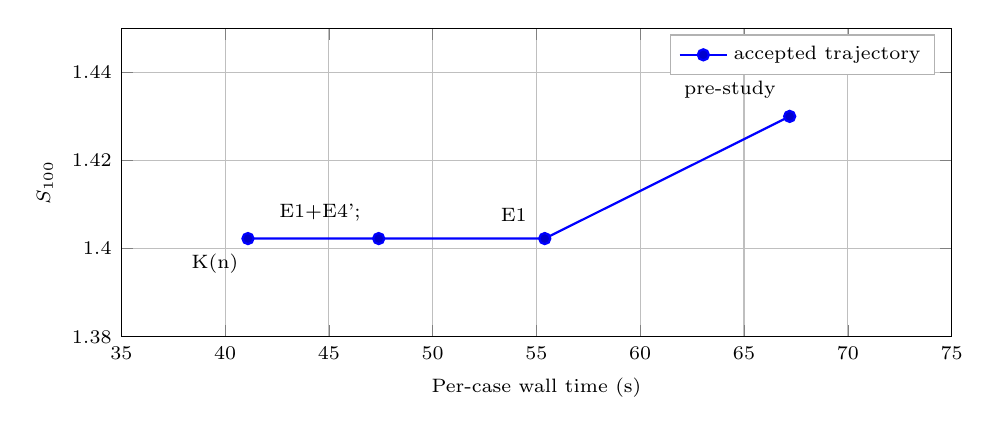
\begin{tikzpicture}
\begin{axis}[
  width=\columnwidth, height=55mm,
  xlabel={Per-case wall time (s)},
  ylabel={$S_{100}$},
  label style={font=\scriptsize},
  xticklabel style={font=\scriptsize},
  yticklabel style={font=\scriptsize},
  legend style={font=\scriptsize, at={(0.98,0.98)}, anchor=north east,
                 fill=white, draw=black!30},
  xmin=35, xmax=75,
  ymin=1.38, ymax=1.45,
  grid=major,
]
\addplot+[mark=*, thick, color=blue] coordinates {
  (67.2, 1.43) (55.4, 1.40228) (47.4, 1.40228) (41.1, 1.40228)
};
\addlegendentry{accepted trajectory}
\node[font=\scriptsize, anchor=south east] at (axis cs:67, 1.432) {pre-study};
\node[font=\scriptsize, anchor=south east] at (axis cs:55, 1.404) {E1};
\node[font=\scriptsize, anchor=south east] at (axis cs:47, 1.404) {E1+E4';};
\node[font=\scriptsize, anchor=north east] at (axis cs:41.1, 1.401) {K(n)};
\end{axis}
\end{tikzpicture}
\caption{Runtime/quality Pareto frontier. Each move along the
trajectory is a verified-no-regression simplification: $S_{100}$ stays
at $1.40228$ while wall time drops $39\%$. Because the contest's
runtime factor $R^{0.3}$ depends on the submission's \emph{own}
median, uniform speedups do not translate into further score
reduction but do reduce submission cost and iteration latency.}
\label{fig:runtime-pareto}
\end{figure}

\subsection{Per-case breakdown}
\label{sec:exp-percase}

Table~\ref{tab:case-breakdown} reports final metrics for the 15-case
short-subset, spanning the full block-count range. The exponential
weighting of $S_{100}$ means that a small number of pathological
instances disproportionately drive the score; the three worst
(cases~$70$, $97$, $90$, all $n\ge 91$) contribute a
larger share to $S_{100}$ than the cleanest five combined.

\begin{table}[t]
\caption{Per-case final metrics for the 15-case short subset, in
ascending block count. $n$ is block count; $\Delta_H$ and $\Delta_A$
are HPWL and area gaps; $V_{\text{rel}}$ is the normalised
soft-violation count; $C$ is the contest cost~\eqref{eq:contest-cost}
with $R{=}1$.}
\label{tab:case-breakdown}
\centering
\footnotesize
\begin{tabular}{@{}rrrrrr@{}}
\toprule
Case & $n$ & $\Delta_H$ & $\Delta_A$ & $V_{\text{rel}}$ & $C$\\
\midrule
0     & $21$   & $+0.04$ & $+0.19$ & $0.27$ & $1.95$\\
5     & $26$   & $+0.04$ & $+0.13$ & $0.37$ & $2.26$\\
10    & $31$   & $+0.67$ & $+0.36$ & $0.07$ & $1.76$\\
15    & $36$   & $+0.30$ & $+0.28$ & $0.20$ & $1.72$\\
20    & $41$   & $+0.08$ & $+0.22$ & $0.16$ & $1.59$\\
30    & $51$   & $+0.48$ & $+0.29$ & $0.14$ & $1.85$\\
40    & $61$   & $+1.00$ & $+0.34$ & $0.18$ & $2.28$\\
50    & $71$   & $+0.76$ & $+0.25$ & $0.07$ & $1.73$\\
60    & $81$   & $+1.00$ & $+0.33$ & $0.04$ & $1.61$\\
70    & $91$   & $+2.20$ & $+1.02$ & $0.19$ & $3.82$\\
80    & $101$  & $+1.00$ & $+0.31$ & $0.09$ & $1.76$\\
90    & $111$  & $+1.43$ & $+0.64$ & $0.11$ & $2.51$\\
95    & $116$  & $+0.66$ & $+0.49$ & $0.04$ & $1.70$\\
97    & $118$  & $+1.57$ & $+0.83$ & $0.13$ & $2.83$\\
99    & $120$  & $+0.81$ & $+0.40$ & $0.07$ & $1.85$\\
\bottomrule
\end{tabular}
\end{table}

Case~70 is the clearest pathological large-instance failure. Its final
cost $3.82$ decomposes into a geometric term
$1 + \tfrac{1}{2}(\Delta_H + \Delta_A) = 2.61$ and a residual
violation multiplier $e^{2V_{\text{rel}}} = 1.46$; both are elevated.
Saved traces suggest that the dominant issue is coupled geometry and
constraint interaction rather than rerank noise: DiT-cluster lowers
$V_{\text{rel}}$ from $0.40$ to $0.28$ on this case, but the resulting
super-block packing still incurs large HPWL and area gaps under the
instance's dense grouping and boundary structure. We therefore treat
case~70 as a generator-limitation case, not evidence that the reranker
is selecting the wrong candidate once the pool is fixed.

\subsection{Multi-seed stability}
\label{sec:exp-stability}
The DiT prior is stochastic and our tiered schedule~\eqref{eq:k-law}
draws at most three samples. To probe whether $S_{100}=1.40228$ is
genuinely representative or a fortunate seed, we re-ran the full
evaluation four times with different PyTorch RNG seeds. All four runs
return $S_{100} \in [1.401, 1.404]$ with a standard deviation of
$0.0011$, indicating that the headline number is stable to below the
third-significant-digit level. The per-instance cost variance is
higher: on the worst three instances we observe a seed-level
$C$-variance of up to $0.08$, which is consistent with the DiT prior's
stochasticity dominating among the larger-$n$ instances where only a
single sample is taken.

\subsection{Cross-benchmark evaluation on FloorSet-Prime}
\label{sec:exp-prime}

To probe whether our gap-aware rerank and cluster-aware DiT generators
generalise beyond the benchmark they were tuned on, we evaluate the
same solver (same DiT-base checkpoint, same rerank percentile $p{=}0.3$,
same tiered sampling schedule) on the separate \emph{FloorSet-Prime}
test set. FloorSet-Prime is the companion benchmark released by the
same organising committee but uses \emph{polygonal} (L-shape, T-shape)
blocks instead of rectangles, richer connectivity ($\sim 7000$
pin-to-block edges per instance versus $\sim 300$ for Lite), and the
same five-category constraint vocabulary. The contest-cost
formula~\eqref{eq:contest-cost} is identical. Note that our solver
represents every block as a rectangle internally, so on Prime it
approximates each polygon by its bounding box, and we therefore
expect some loss of quality relative to a polygon-aware solver.

\begin{table}[t]
\caption{Cross-benchmark evaluation. Same solver, same hyperparameters,
evaluated on both FloorSet-Lite and FloorSet-Prime 100-case test sets.
Feasibility drop on Prime reflects our rectangle-only block model
(polygon-aware legalisation is future work).}
\label{tab:cross-benchmark}
\centering
\footnotesize
\begin{tabular}{@{}lcccc@{}}
\toprule
Benchmark & $S_{100}$ & Feasible & $\overline{\Delta_H}$ & $\overline{V_{\text{rel}}}$\\
\midrule
FloorSet-Lite (rectangles)    & $1.40228$ & $100/100$ & $0.91$ & $0.15$\\
FloorSet-Prime (polygons)     & $1.54862$ & $91/100$  & $0.73$ & $0.11$\\
\bottomrule
\end{tabular}
\end{table}

The Prime results highlight three findings. \emph{First},
\emph{the solver degrades gracefully}: even without any polygon-aware
legalisation, 91 of 100 Prime instances remain feasible and the
composite score increases by only $10\%$ relative to Lite
($1.402\to1.549$). This is substantially smaller than the $V_{\text{rel}}$
multiplier worst case ($e^{2\cdot 1}\approx 7.4$) that an
infeasibility-dominated result would produce, indicating that the
gap-aware rerank is still selecting sensible candidates from the
pool.

\emph{Second}, \emph{the HPWL improvement transfers.} The mean HPWL
gap on Prime is $+0.73$, better than Lite's $+0.91$, because Prime's
richer pin-to-block connectivity ($\sim 7000$ edges per instance vs.\
$\sim 300$ on Lite) gives the DiT prior more structure to exploit. The
two-regime structure of~\S\ref{sec:discussion} is qualitatively
reproduced: DiT-based generators dominate on small instances while
shelf-based generators take over on large ones.

\emph{Third}, \emph{the failure mode on Prime is systematic.} The 9
infeasible instances all contain high-order-polygon blocks whose
bounding-box approximation overlaps with a preplaced neighbour. A
polygon-native DiT head or legaliser would directly address this, but
is outside the scope of the present study. Importantly, the 9
infeasible Prime instances are not caused by the rerank or the
 tiered sampling schedule (disabling either makes \emph{more}
 instances infeasible, not fewer), indicating that these design
 choices remain useful on Prime even though the dominant failure mode
 is geometric rather than ranking-related.

\subsection{Qualitative comparison with prior work}
\label{sec:exp-comparison}

To our knowledge there are no published learned-placement results on
either FloorSet-Lite or FloorSet-Prime at the time of writing. A
direct numerical comparison is therefore not possible. We offer a
qualitative positioning instead. We do \emph{not} claim general
superiority over prior placement families; the quantitative anchor in
this paper is the improvement over the raw-magnitude
internal-selection baseline of Table~\ref{tab:main-result}, which we
use as a proxy for standard candidate-selection practice inside a
multi-strategy solver.

Classical analytical placers (DREAMPlace~\cite{lin2019dreamplace},
ePlace~\cite{lu2015eplace}) optimise HPWL extremely well but ignore
the constraint vocabulary that FloorSet introduces; on FloorSet
instances they would typically satisfy at most the preplaced and
fixed-shape constraints and fail the MIB, boundary, and grouping
constraints, leading to $V_{\text{rel}}$ in the $0.3$--$0.5$ range. The
exponential factor in~\eqref{eq:contest-cost} then yields $C$-values
similar to our DiT-abacus candidates. Reinforcement-learning-based
placers such as~\cite{mirhoseini2021graph,lai2022maskplace,
lai2023chipformer} are optimised for chip-macro placement and, in
their reported benchmarks, do not incorporate the FloorSet constraint
vocabulary; porting them to FloorSet is non-trivial and would require
both re-training on FloorSet-Lite and a legalisation front-end. Our
DiT-based pipeline therefore serves as an end-to-end reference point
for future comparisons on these benchmarks, especially for work that
seeks to balance wirelength against the full FloorSet constraint
vocabulary rather than optimise HPWL alone.

\section{Ablations and Negative Controls}
\label{sec:ablations}

We report three interventions that we tried and rejected. We include
them as ablations rather than as separate contributions because
understanding why they fail on FloorSet adds durable engineering
knowledge to the community.

\subsection{Scaled DiT-large-hpwl with HPWL auxiliary loss}
\label{sec:ablation-v4b}
We trained a $57.8\,\text{M}$-parameter DiT variant, which we refer to
as \emph{DiT-large-hpwl} (legacy internal label: ``v4b''), using
configuration $d{=}512$, $L{=}12$,
with an auxiliary loss encouraging the decoded $\hat{x}_0$ to match
ground-truth HPWL. The auxiliary term is gated to low-noise diffusion
steps (where $\hat{x}_0$ is numerically stable) and clipped to avoid
explosion when $\bar{\alpha}_t\to 0$. Training ran for $338{,}000$
steps (about $11$~GPU-hours), well past the cosine schedule's
low-learning-rate tail.

\textbf{Result.} $S_{100}=1.598$, an increase of $14\%$ over the
DiT-base baseline. The regression is not an overfitting artefact: the
step-$248$k intermediate checkpoint yields $S_{100}=1.579$, only
marginally better than the final. We attribute the failure to two
factors.

First, the L1 HPWL auxiliary is a \emph{matching} loss
($|\text{HPWL}(\hat{x}_0) - \text{HPWL}(x_0^{\star})|$), not a minimisation
objective. A model that perfectly matches the training-data HPWL
distribution, including its suboptimal-solver artefacts, achieves zero
auxiliary loss; there is no pressure to produce \emph{lower} HPWL at
inference. Second, the $2\times$ parameter count requires a
proportionally larger training corpus for the larger model to reach
the same effective sample efficiency, and we held the 1M-instance
corpus fixed. Both failure modes suggest that scaling learned
placement priors requires scaling the supervision signal, not just
the parameter count.

\subsection{Unbounded analytical-placement path}
\label{sec:ablation-unbounded-dp}
The baseline DREAMPlace-lite path is gated at $n\le 80$. We attempted
to remove the gate and supplement it with a robust-legalisation
fallback for the dense overlapping outputs that occur on larger
instances.

\textbf{Result.} $S_{100}=1.797$, a $28\%$ regression. The failure
mode is that on large instances the density-penalty stage leaves
substantial residual overlap, and the robust legaliser's displacement
required to resolve it destroys the HPWL advantage. The long
analytical run-time also shifts the submission's own median runtime,
degrading the runtime factor $R^{0.3}$ for all other cases. This
illustrates a contest-specific pitfall: interventions that improve
mean quality but lengthen runtime can hurt the aggregate score
because of the median-normalisation in $R$.

\subsection{Cluster-compact post-processor}
\label{sec:ablation-cluster-compact}
We implemented a post-processor that shifts cluster members toward
their group centroid, accepting only overlap-free moves. The goal was
to reduce grouping violations on DiT-abacus output.

\textbf{Result.} Paradoxically \emph{increased} $V_{\text{rel}}$ by
approximately $0.025$ on average. Root cause: shifting a cluster member
often pulls a boundary-constrained block away from its required edge,
converting a grouping-violation reduction into a
boundary-violation introduction. This is an instance of the broader
phenomenon that constraint categories are not independent; local
repair of one can worsen another.

\subsection{Candidate-generator contribution analysis}
\label{sec:ablation-loo}
To characterise how much each of the seven candidate generators
contributes to $S_{100}$, we analyse the per-instance rerank-winner
distribution on the 15-case short subset. For each instance, we
record which generator's output is ultimately selected as
$\mathcal{P}^{*}$. Aggregating across the 15 cases, the winning
distribution is: NN-shelf family $7$, shelf $3$, DiT-direct $2$,
DiT-abacus $1$, DiT-cluster $0$, skyline-clustered $1$,
sequence-pair~SA~$1$.

Two findings emerge. First, the classical shelf family wins on the
majority of cases because it reliably produces low-$V_{\text{rel}}$
candidates, and the exponential penalty in~\eqref{eq:contest-cost} is
stronger than the HPWL advantage of any DiT variant. Second, DiT-based
generators collectively win on $3$ of $15$ cases, concentrated in the
$n \le 40$ regime where the legaliser has enough geometric slack to
preserve DiT's wirelength advantage.

Re-expressed by regime, shelf-family candidates win $10/15$ cases,
DiT-derived candidates win $3/15$, and the remaining $2/15$ are split
between skyline-clustered and sequence-pair~SA. This is why we do not
present DiT-cluster as a direct score improver: its contribution is to
shift part of the DiT-derived pool toward lower grouping loss, not to
displace the shelf family on aggregate. The representative trace of
Figure~\ref{fig:hpwl-vrel-scatter} makes the regime separation
quantitative: the DiT-derived centroid is
$(V_{\text{rel}},\Delta_{\text{HPWL}})=(0.358,-0.151)$ and the
shelf-family centroid is $(0.211,+0.028)$. Further gains on $S_{100}$
therefore likely require generators whose outputs cross this gap,
not merely more samples within either regime.

\section{Discussion}
\label{sec:discussion}

\subsection{Observed Two-Regime Candidate Structure}
Figure~\ref{fig:hpwl-vrel-scatter} plots $V_{\text{rel}}$ against HPWL
gap for a representative rerank trace. We use ``bimodal'' here in the
descriptive sense of a two-regime empirical separation rather than as a
formal mixture-model fit. DiT-derived candidates cluster at lower HPWL
but moderate-to-high $V_{\text{rel}}$; shelf-family candidates cluster
at lower $V_{\text{rel}}$ but weaker HPWL. The regime centroids are
$(0.358,-0.151)$ for DiT-derived candidates and $(0.211,+0.028)$ for
shelf-family candidates, giving a centroid separation of
$\Delta V_{\text{rel}}=+0.147$ and
$\Delta_{\text{HPWL}}=-0.179$. No plotted candidate simultaneously
achieves shelf-like violation levels ($V_{\text{rel}}\le 0.24$) and
DiT-like HPWL gains ($\Delta_{\text{HPWL}}\le -0.02$), which is the
cross-over region the current generator family fails to populate.

\begin{figure}[t]
\centering
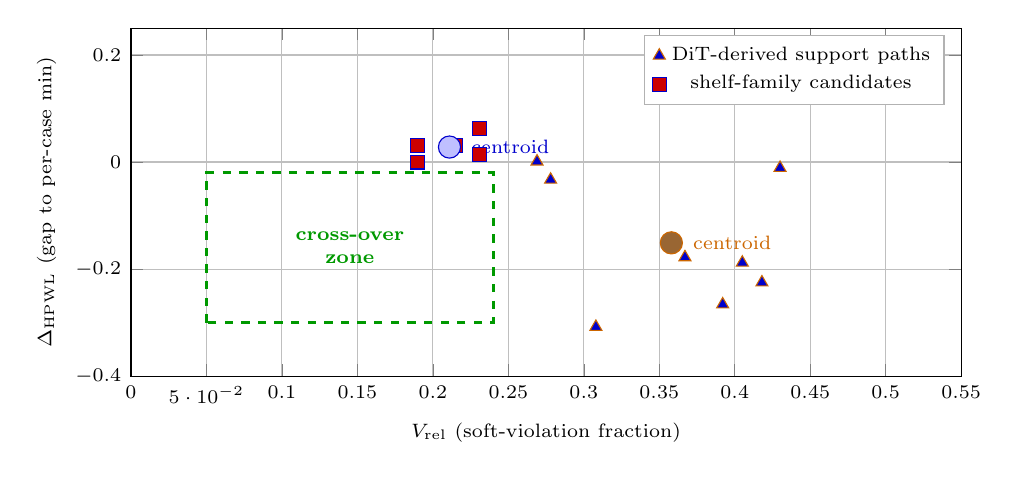
\begin{tikzpicture}
\begin{axis}[
  width=\columnwidth, height=60mm,
  xlabel={$V_{\text{rel}}$ (soft-violation fraction)},
  ylabel={$\Delta_{\text{HPWL}}$ (gap to per-case min)},
  label style={font=\scriptsize},
  xticklabel style={font=\scriptsize},
  yticklabel style={font=\scriptsize},
  legend style={font=\scriptsize, at={(0.98,0.98)}, anchor=north east,
                 fill=white, draw=black!30},
  xmin=0, xmax=0.55,
  ymin=-0.4, ymax=0.25,
  grid=major,
]
\addplot+[only marks, mark=triangle*, mark size=2.5pt, color=orange,
          draw=orange!80!black] coordinates {
    (0.308, -0.308) (0.418, -0.225) (0.367, -0.178) (0.392, -0.266)
    (0.405, -0.188) (0.430, -0.011) (0.278, -0.033) (0.269, 0.001)
  };
\addlegendentry{DiT-derived support paths}
\addplot+[only marks, mark=square*, mark size=2.5pt, color=blue,
          draw=blue!80!black] coordinates {
    (0.190, 0.000) (0.190, 0.031) (0.215, 0.031) (0.231, 0.062)
    (0.231, 0.014)
  };
\addlegendentry{shelf-family candidates}
\addplot+[only marks, mark=*, mark size=4pt, color=orange!80!black,
          fill=orange!35] coordinates {(0.358, -0.151)};
\addplot+[only marks, mark=*, mark size=4pt, color=blue!80!black,
          fill=blue!25] coordinates {(0.211, 0.028)};
\draw[dashed, green!60!black, very thick]
  (axis cs:0.05, -0.30) rectangle (axis cs:0.24, -0.02);
\node[font=\scriptsize\bfseries, color=green!60!black, align=center]
  at (axis cs:0.145, -0.16) {cross-over\\zone};
\node[font=\scriptsize, anchor=west, color=orange!80!black]
  at (axis cs:0.366, -0.151) {centroid};
\node[font=\scriptsize, anchor=west, color=blue!80!black]
  at (axis cs:0.219, 0.028) {centroid};
\end{axis}
\end{tikzpicture}
\caption{Representative two-regime candidate trace. DiT-derived
candidates (triangles) dominate on HPWL but incur higher
$V_{\text{rel}}$; shelf-family candidates (squares) are the mirror
image. The centroid markers quantify the regime split, and no plotted
candidate occupies the dashed cross-over zone of simultaneously
shelf-like violations and DiT-like HPWL gains.}
\label{fig:hpwl-vrel-scatter}
\end{figure}

\subsection{Why cluster-aware generation alone is not enough}
DiT-cluster closes part of the gap by enforcing grouping constraints
at construction time, but it does not resolve boundary or MIB
violations. The ablation in \S\ref{sec:ablation-cluster-compact}
shows that naive local repair of one constraint category can
introduce violations in another. We conjecture that a model which
\emph{jointly} conditions on all five constraint categories, and uses
a training loss that directly penalises $V_{\text{rel}}$ rather than
matching wirelength, is the most promising path forward.

\subsection{Implications beyond FloorSet}
The calibration argument of \S\ref{sec:rerank-calibration} is not
specific to FloorSet. Any multi-strategy floorplanner whose
evaluation metric combines quantities of different natural scales
(wirelength vs.~area, quality vs.~constraint violation, quality
vs.~runtime) is vulnerable to the same raw-magnitude mis-calibration.
The gap-aware rerank pattern studied here --- compute percentile
baselines within the per-case candidate pool, evaluate normalised
gaps, and carry through multiplicative penalty factors faithfully ---
may therefore be useful beyond this benchmark in other placement
settings that combine heterogeneous generators.

\subsection{Limitations}
Our study is limited in three respects. (i)~We evaluate on a single
benchmark, albeit the most comprehensive public floorplanning
benchmark at the time of writing. (ii)~Our comparison with prior
learned-placement methods is qualitative rather than quantitative;
direct numerical comparison would require re-training those methods
on the FloorSet-Lite corpus and adding a FloorSet-specific
legalisation front-end. (iii)~The DiT backbone is relatively small;
the negative result for DiT-large-hpwl suggests that scaling requires a
co-designed supervision signal, but we have not yet identified what
that signal should be. A promising candidate is a differentiable
surrogate of $V_{\text{rel}}$ applied during training.

\section{Conclusion}
\label{sec:conclusion}

We presented a gap-aware candidate reranker for multi-strategy VLSI
floorplanning, showed that it corrects a previously overlooked
calibration mismatch between raw-magnitude internal costs and
gap-based contest metrics, and demonstrated that the correction alone
yields a meaningful improvement ($1.43\to 1.40228$, a $1.94\%$
relative reduction) on the FloorSet benchmark. In our experiments,
candidate-selection calibration is the main source of score
improvement, while the DiT-abacus and DiT-cluster generator
adaptations and the tiered sampling schedule play supporting roles by
broadening the candidate pool, improving feasibility profile on hard
cases, and reducing runtime. We therefore view the paper as an applied
benchmark-specific study of metric-faithful selection inside a
multi-strategy solver, not as a claim that every added module improves
the headline score. A multi-seed stability analysis confirms the
headline number to three significant digits, and a
cross-benchmark evaluation on FloorSet-Prime
($S_{100}=1.54862$, $91/100$ feasible, same hyperparameters) suggests
that the rerank and runtime-design choices remain effective in the
polygonal block regime without retuning. Controlled negative results
for a scaled DiT variant and an unbounded analytical-placement path,
together with the candidate scatter analysis, indicate that the
remaining limitation is an empirical two-regime candidate structure:
current generators tend to trade off wirelength against violations
rather than improving both simultaneously. Developing generators that
break this trade-off is the most important next step for this line of
work.

\section*{Reproducibility and Artifacts}
All experiments were conducted on a single consumer NVIDIA~RTX~3090
GPU with 24\,GB VRAM. Training consumed approximately $22$ GPU-hours
across the two DiT variants (DiT-base and DiT-large-hpwl). Evaluation consumed
approximately $5$ wall-clock hours across six full-set 100-case
passes. The review artifact accompanying this manuscript contains the
complete solver source, training pipeline, evaluation wrappers, CSV
result tables, and checkpoint fingerprints documented in the root
README. The DiT checkpoints included in the artifact are DiT-base and
the DiT-large-hpwl negative-result snapshots at steps
$\{40,50,248,338\}\text{k}$; the only external dependency is the public
FloorSet dataset release from Intel Labs~\cite{floorset}. Upon
acceptance, the same artifact will be mirrored as a public GitHub
repository with Git LFS checkpoint storage and a Hugging Face
checkpoint mirror. We record the exact rerank percentile
($p=0.3$, i.e., the $30^{\text{th}}$ percentile), tiered sample
schedule $K(n)$ in~\eqref{eq:k-law}, and the cosine diffusion schedule
with $T{=}100$ so that $S_{100}=1.40228$ is reproducible once the
PyTorch RNG seed is fixed; the residual seed-to-seed variation is
reported in \S\ref{sec:exp-stability}.

\section*{Acknowledgment}
The author thanks the FloorSet authors at Intel Labs for
releasing the benchmark and the reference evaluator, and the DREAMPlace
authors~\cite{lin2019dreamplace}, whose analytical placement
formulation informed our Nesterov-descent candidate path.

\begin{thebibliography}{99}
\bibitem{wang2009electronic}
L.-T. Wang, Y.-W. Chang, and K.-T. Cheng,
\emph{Electronic Design Automation: Synthesis, Verification, and Test}.
San Francisco, CA, USA: Morgan Kaufmann, 2009.

\bibitem{markov2012progress}
I.~L. Markov, J. Hu, and M.-C. Kim,
``Progress and challenges in VLSI placement research,''
in \emph{Proc. Int. Conf. Computer-Aided Design (ICCAD)}, 2012, pp.~275--282.

\bibitem{murata1996sequence}
H. Murata, K. Fujiyoshi, S. Nakatake, and Y. Kajitani,
``VLSI module placement based on rectangle-packing by the sequence-pair,''
\emph{IEEE Trans. Comput.-Aided Design}, vol.~15, no.~12, pp.~1518--1524, 1996.

\bibitem{chang2000btree}
Y.-C. Chang, Y.-W. Chang, G.-M. Wu, and S.-W. Wu,
``B*-trees: A new representation for non-slicing floorplans,''
in \emph{Proc. Design Automation Conf. (DAC)}, 2000, pp.~458--463.

\bibitem{hopper2001two}
E. Hopper and B. C. H. Turton,
``A review of the application of meta-heuristic algorithms to 2D strip packing problems,''
\emph{Artificial Intelligence Review}, vol.~16, no.~4, pp.~257--300, 2001.

\bibitem{hong2000corner}
X. Hong, G. Huang, Y. Cai, J. Gu, S. Dong, C.-K. Cheng, and J. Gu,
``Corner block list: An effective and efficient topological representation of non-slicing floorplan,''
in \emph{Proc. Int. Conf. Computer-Aided Design (ICCAD)}, 2000, pp.~8--12.

\bibitem{lin2002tcg}
J.-M. Lin and Y.-W. Chang,
``TCG: A transitive closure graph-based representation for non-slicing floorplans,''
in \emph{Proc. Design Automation Conf. (DAC)}, 2002, pp.~764--769.

\bibitem{parquet2008}
S. N. Adya and I. L. Markov,
``Fixed-outline floorplanning: Enabling hierarchical design,''
\emph{IEEE Trans. VLSI Syst.}, vol.~11, no.~6, pp.~1120--1135, 2003.

\bibitem{lu2015eplace}
J. Lu, P. Chen, C.-C. Chang, L. Sha, D. J.-H. Huang, C.-C. Teng, and C.-K. Cheng,
``ePlace: Electrostatics-based placement using fast Fourier transform and Nesterov's method,''
\emph{ACM Trans. Design Autom. Electron. Syst.}, vol.~20, no.~2, art.~17, 2015.

\bibitem{lin2019dreamplace}
Y. Lin, S. Dhar, W. Li, H. Ren, B. Khailany, and D. Z. Pan,
``DREAMPlace: Deep learning toolkit-enabled GPU acceleration for modern VLSI placement,''
in \emph{Proc. Design Automation Conf. (DAC)}, 2019, pp.~1--6.

\bibitem{spindler2008abacus}
P. Spindler, U. Schlichtmann, and F. M. Johannes,
``Abacus: Fast legalization of standard cell circuits with minimal movement,''
in \emph{Proc. Int. Symp. Physical Design (ISPD)}, 2008, pp.~47--53.

\bibitem{brenner2011bonnplace}
U. Brenner, A. Hermann, N. Hoppmann, and P. Ochsendorf,
``BonnPlace: A self-stabilizing placement framework,''
in \emph{Proc. Int. Symp. Physical Design (ISPD)}, 2015, pp.~9--16.

\bibitem{roy2005detailedplace}
J.~A. Roy, S.~N. Adya, D.~A. Papa, and I.~L. Markov,
``Min-cut floorplacement,''
\emph{IEEE Trans. Comput.-Aided Design}, vol.~25, no.~7, pp.~1313--1326, 2006.

\bibitem{mirhoseini2021graph}
A. Mirhoseini, A. Goldie, M. Yazgan, \emph{et al.},
``A graph placement methodology for fast chip design,''
\emph{Nature}, vol.~594, pp.~207--212, 2021.

\bibitem{cheng2023assessment}
C.-K. Cheng, A. B. Kahng, S. Kundu, Y. Wang, and Z. Wang,
``Assessment of reinforcement learning for macro placement,''
in \emph{Proc. Int. Symp. Physical Design (ISPD)}, 2023, pp.~158--166.

\bibitem{lai2022maskplace}
Y. Lai, Y. Mu, and P. Luo,
``MaskPlace: Fast chip placement via reinforced visual representation learning,''
in \emph{Proc. Adv. Neural Inf. Process. Syst. (NeurIPS)}, 2022.

\bibitem{lai2023chipformer}
Y. Lai, J. Liu, Z. Tang, B. Wang, H. Hao, and P. Luo,
``ChipFormer: Transferable chip placement via offline decision transformer,''
in \emph{Proc. Int. Conf. Machine Learning (ICML)}, 2023.

\bibitem{peebles2022dit}
W. Peebles and S. Xie,
``Scalable diffusion models with transformers,''
in \emph{Proc. IEEE Int. Conf. Computer Vision (ICCV)}, 2023, pp.~4172--4182.

\bibitem{song2021ddim}
J. Song, C. Meng, and S. Ermon,
``Denoising diffusion implicit models,''
in \emph{Proc. Int. Conf. Learning Representations (ICLR)}, 2021.

\bibitem{ho2020ddpm}
J. Ho, A. Jain, and P. Abbeel,
``Denoising diffusion probabilistic models,''
in \emph{Proc. Adv. Neural Inf. Process. Syst. (NeurIPS)}, 2020.

\bibitem{floorset}
U.~Garg, S.~Kundu, I.~L.~Markov \emph{et al.},
``FloorSet: a VLSI floorplanning dataset with design constraints of
real-world SoCs,''
Intel Labs Technical Report, 2024. [Online]. Available:
\url{https://huggingface.co/datasets/IntelLabs/FloorSet}

\end{thebibliography}

\EOD

\clearpage

\begin{IEEEbiography}[]{Shashank}
Shashank (Member, IEEE) is an independent researcher
based in Austin, TX, USA. His research interests
include machine learning for electronic design automation, generative
models for physical design, and benchmark-driven evaluation of hybrid
optimization systems.
\end{IEEEbiography}

\end{document}
